\documentclass[blue]{beamer}
%\documentclass[handout]{beamer}

%\beamerboxesdeclarecolorscheme{alert}{brown}{brown!25!averagebackgroundcolor}

\usepackage{beamerthemeshadow}
\usepackage[ngerman]{babel}
\usepackage[ansinew]{inputenc}
\usepackage{html,makeidx}

\hypersetup{colorlinks=true,pagecolor=blue,urlcolor=blue} % linkcolor=green,filecolor=red

%%%%%%%%%%%%%%%%%%%%%%%%%%%%%%%%%%%%%%%%%%%%%%%%%%%%%%%%%%%%%%%%%%%%%%%%%%%%%%%%%%%%
%%%%%%%%%%%%%%%%%%%%%%%%%%%%%%%%%%%%%%%%%%%%%%%%%%%%%%%%%%%%%%%%%%%%%%%%%%%%%%%%%%%%

\title{METANET - Distributed Interactive Knowledge Network}
\institute[META-D.O.N]{META-D.O.N\\Association for Cultural Substitution Services}
\author{Hannes Weingartner}
\date{April 17, 2010}

\begin{document}
\frame{\titlepage}

% no entry in TOC but in the navigation bar
%\section*{overview}
\setcounter{tocdepth}{1}
\frame{\tableofcontents}


%%%%%%%%%%%%%%%%%%%%%%%%%%%%%%%%%%%%%%%%%%%%%%%%%%%%%%%%%%%%%%%%%%%%%%%%%%%%%%%%%%%%
%%%%%%%%%%%%%%%%%%%%%%%%%%%%%%%%%%%%%%%%%%%%%%%%%%%%%%%%%%%%%%%%%%%%%%%%%%%%%%%%%%%%


\section{project}
\subsection{introduction}
\frame
{
\frametitle{\textbf{project introduction}}
\begin{itemize}
\item \textbf{metanet:} the technical aspect of a project of the \textbf{Meta-D.O.N Association}: sociocultural studies in Serbia called \textbf{New[B]Order} - \htmladdnormallink{http://www.meta-don.org/newborder/}{http://www.meta-don.org/newborder/}
\item project on the topography of the centre-periphery-complex in post-communist Eastern Europe
\item metastatic penetration of social spaces scientifically measured to create quantitative and qualitative indicators for social disintegration
\end{itemize}
}

\frame
{
\frametitle{\textbf{project introduction}}
\begin{itemize}
	\item e.g. indicators
	\begin{itemize}
		\item privatization aspects of companies in Serbia - \textbf{Freedom Fighters Collective} (\htmladdnormallink{http://www.freedomfight.net/cms/}{http://www.freedomfight.net/cms/})
		\item subversive signs of the periphery
		\item turbo folk politics
	\end{itemize}
	\item capture indicators cartographically with a link to a visual semantic database
	\item concept of an interactive geo-spatial \textbf{knowledge network}
	\item web application based on \textbf{free- and open source software components}
\end{itemize}
}


\subsection{goal}
\frame
{
\frametitle{\textbf{project goal}}
\begin{itemize}
\item providing a tool for individuals and communities to get \textbf{connected to complex relationships of scientfic measurement} with cartographical aspects
\item receiving a better \textbf{overall view of knowledge related to public areas} which can be meaningful for exploring topics of interests through the user
\item \textbf{flexiblity in usage:} generic tool for scientific research projects
\item \textbf{administration:} intuitive CMS interface for researchers
\item smart algorithms for finding similarities/references between artifacts
\item \textbf{usability:} advanced hardware and software interfaces to the user (e.g for exhibitions)
\end{itemize}
}


\subsection{domains}
\frame
{
\frametitle{\textbf{project domains}}
\begin{itemize}
\item project consists of three \textbf{technical domains} 
\item \textbf{metablog - artifacts input:}
  \begin{itemize}
    \item text, sound, images, an mm data through web-based CMS
    \item mobile devices for geo-tagged content input
  \end{itemize}
\item \textbf{metamap:} 2D map for customized geographical representation of artifacts and transformation processes between them
\item \textbf{metaspace:} 2D/3D semantic graph/subgraph associated with map artifacts for mapping the degree of connectivity between them
\end{itemize}
}

\frame
{
\frametitle{\textbf{project domains}}
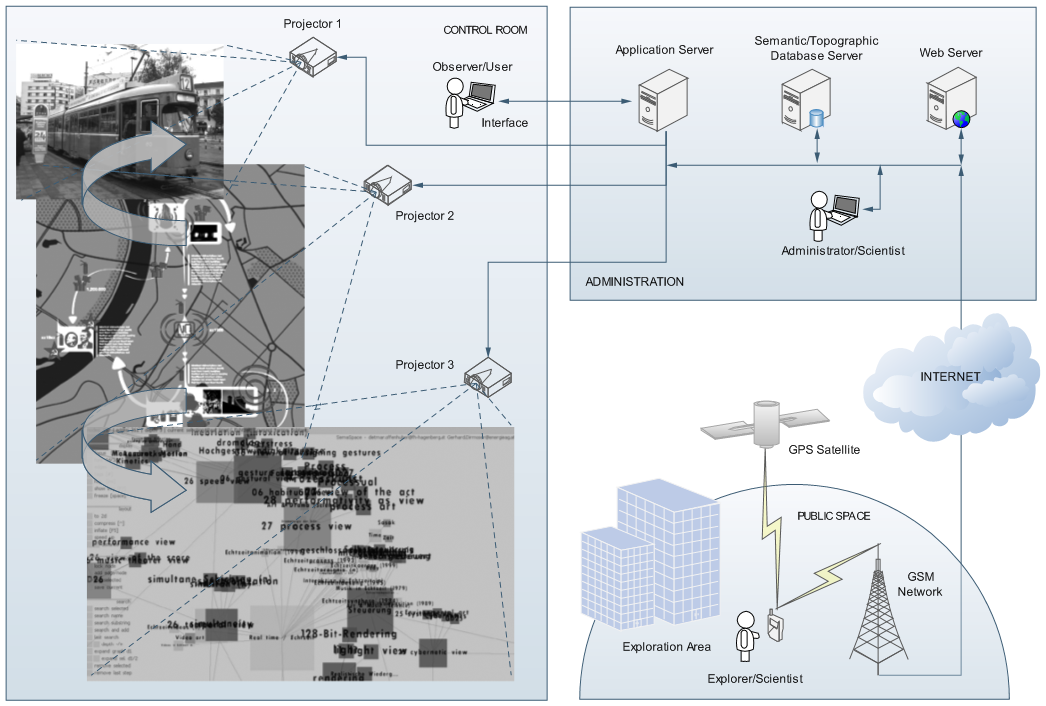
\includegraphics[width=0.85\textwidth]{bin/domains/domains.png}
}


\subsection{challenges}
\frame
{
\frametitle{\textbf{project challenges}}
\begin{itemize}
	\item \textbf{metaspace hardware HCI} design and implementation for a seamless exploration of data in the semantic space - extension to keyboard and mouse 
	\item \textbf{customization of map} design and implementation of interactive icons and transformations -  extendable map APIs
	\item \textbf{intuitive administration} and performative web CMS interface for knowledge workers - ajax based server interaction
	\item \textbf{data consistency} between metamap and metaspace - network interface and structured graph datasets for synchronization
	\item \textbf{complex algorithms} for dependency calculation based on meta data and severity - generating an ontology of data
\end{itemize}
}


\subsection{technologies}
\frame
{
\frametitle{\textbf{project technologies}}
\begin{itemize}
\item \textbf{main aspect:} utilization of proofed open-source/free tools for adapting them to our needs  
\item \textbf{dependencies on tools:}
  \begin{itemize}
    \item \textbf{Semaspace} (\htmladdnormallink{http://residence.aec.at/didi/FLweb/}{http://residence.aec.at/didi/FLweb/})
    \item \textbf{OpenStreetMap} aka OSM (\htmladdnormallink{http://www.openstreetmap.org/}{http://www.openstreetmap.org/})
    \item \textbf{Google Web Toolkit 2.0} aka GWT (\htmladdnormallink{http://code.google.com/webtoolkit/}{http://code.google.com/webtoolkit/})
  \end{itemize}
\item \textbf{language:}
	\begin{itemize}
		\item Java
		\item Java Script
	\end{itemize}
\end{itemize}
}

%%%%%%%%%%%%%%%%%%%%%%%%%%%%%%%%%%%%%%%%%%%%%%%%%%%%%%%%%%%%%%%%%%%%%%%%%%%%%%%%%%%%
%%%%%%%%%%%%%%%%%%%%%%%%%%%%%%%%%%%%%%%%%%%%%%%%%%%%%%%%%%%%%%%%%%%%%%%%%%%%%%%%%%%%

% TODO research:  knowledge network, maps
\section{knowledge networks}
\subsection{theory}
\frame
{
\frametitle{\textbf{knowledge networks theory}}
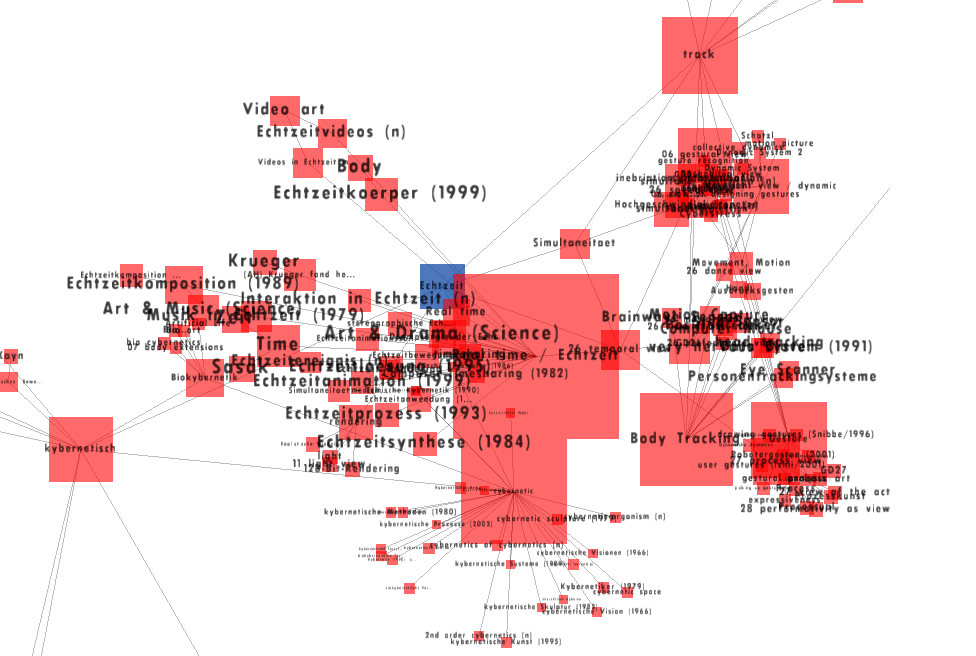
\includegraphics[width=0.85\textwidth]{bin/semaspace/semaspace.png}
}

\frame
{
\frametitle{\textbf{knowledge networks theory}}
\begin{itemize}
	\item \textbf{knowledge representation and visual interfaces} (\htmladdnormallink{http://media.lbg.ac.at}{http://media.lbg.ac.at})
	\begin{itemize}
		\item \textbf{semantic networks} become readable if their structures are described through an ontology
		\item \textbf{ontologies} are abstract knowledge models for describing used concepts and their possible relationships
		\item interactive tools realize the generation of \textbf{smooth image of information} to take ambiguity and complexity into account
	\end{itemize}
\end{itemize}
}




%%%%%%%%%%%%%%%%%%%%%%%%%%%%%%%%%%%%%%%%%%%%%%%%%%%%%%%%%%%%%%%%%%%%%%%%%%%%%%%%%%%%
%%%%%%%%%%%%%%%%%%%%%%%%%%%%%%%%%%%%%%%%%%%%%%%%%%%%%%%%%%%%%%%%%%%%%%%%%%%%%%%%%%%%


\section{semaspace}
\subsection{outline}
\frame
{
\frametitle{\textbf{semaspace outline}}
\begin{itemize}
	\item \textbf{fast OpenGL accelerated graph editor and browser} for large knowledge networks with more than 10000 text-fields
	\item developed by \textbf{Dietmar Offenhuber and Gerhard Dirmoser} - Ludwig Boltzmann Institute for Media Art Research
	\item \textbf{interactive graph layout} in 2D and 3D
	\item 'semaspace fills the gap between complex tools for network analysis and simple graph editors or mind-mapping tools' (Dirmoser)
	\item Gerhard Dirmoser creates complex large-scale wall diagrams on topics like \textbf{25 years of ARS Electronica or Performance Art} (2003)
\end{itemize}
}

% TODO research: virtools technical + developers
\frame
{
\frametitle{\textbf{semaspace outline}}
\begin{itemize}
	\item manually \textbf{define the nodes overall shape} of the network by placing and subsequently locking the position of individual nodes
	\item \textbf{nodes} can incorporate data such as images, sound and text (added while navigating the graph)
	\item GUI for \textbf{web clients} and \textbf{exhibitions}
	\item \textbf{Java SWT} desktop application
	\item embedding into web clients with \textbf{virtools webplayer}
\end{itemize}
}

\subsection{dependencies}
\frame
{
\frametitle{\textbf{semaspace dependencies}}
\begin{itemize}
	\item \textbf{JOGL:} open source Java binding to OpenGL API from Sun (for harware supported 3D graphics)
	\item \textbf{JFTGL:} java based lib for accessing tt fonts within OpengGL
	\item \textbf{Apache batik SVG toolkit:} open source Java based toolkit for using images in the SVG format (XML based)
	\item \textbf{\htmladdnormallink{semaspace demo}{file:///C:/Users/hn/Workspace-Java/metanet/files/presentation/bin/semaspace/web-demo/semaspace.html}}
\end{itemize}
}


\subsection{extensions}
\frame
{
\frametitle{\textbf{semaspace extensions}}
\begin{itemize}
	\item \textbf{video nodes}
	\item \textbf{remote graph access and manipulation} through network connection and tagged datasets
	\item research and implementation of \textbf{extending hardware interfaces} for browsing
		\begin{itemize}[<+-|alert@+>]
			\item browsing (zoom, rotation)
			\item 2D/3D
			\item fog
			\item freeze
			\item node distance
		\end{itemize}
\end{itemize}
}


%%%%%%%%%%%%%%%%%%%%%%%%%%%%%%%%%%%%%%%%%%%%%%%%%%%%%%%%%%%%%%%%%%%%%%%%%%%%%%%%%%%%
%%%%%%%%%%%%%%%%%%%%%%%%%%%%%%%%%%%%%%%%%%%%%%%%%%%%%%%%%%%%%%%%%%%%%%%%%%%%%%%%%%%%

\section{openstreetmap}
\subsection{outline}
\frame
{
\frametitle{\textbf{OSM outline}}
\begin{itemize}
	\item \textbf{OSM: open source map solution} for web clients
	\item everyone can extend the map
	\item collecting GPS coordinates
	\item like wikipedia for maps
	\item \textbf{no legal or technical restrictions} on their use - full creativity
	\item other implementations do not allow highly customized overlays
\end{itemize}
}

\subsection{strategy}
\frame
{
\frametitle{\textbf{OSM creating data}}
\begin{itemize}
	\item \textbf{creating OSM data} with OSM map editors:
	\begin{itemize}
			\item java OSM (JOSM) - desktop app
			\item potlatch - flash
			\item merkaartor - for UNIX, WIN, MAC
	\end{itemize}
	\item \textbf{adding tags} (node, linear, area) for OSM data do be rendered and upload
	\item \textbf{slippy map:} OSM default web interface for browsing rendered OSM data
\end{itemize}
}

\frame
{
\frametitle{\textbf{OSM rendering}}
\begin{itemize}
\item \textbf{generating rendered graphics} on own computer by using tools:
	\begin{itemize}
			\item \textbf{kosmos:} lightweight OSM map rendering platform for WIN
			\item \textbf{osmarender:} rendering platform for generating SVG image for OSM data based on XSLT
			\item \textbf{mapnik:} opensource toolkit in C++ and python, all OS platforms
			\begin{itemize}
				\item default for OSM - mapnik renders 256 x 256 px tiles served from the OSM tile server
				\item XML file holds rendering props like color, withs of lines, etc.
				\item rendered tiles are referenced by URLs through JS from web client
				\item raw OSM data can be downloaded for setting up an own tile server (e.g. planet.osm)
				\item uses PostgreSQL / PostGIS as spatial database (osm2pgsql converter)
		\end{itemize}
	\end{itemize}
\end{itemize}
}

\subsection{embedding}
\frame
{
\frametitle{\textbf{OSM embedding}}
\begin{itemize}
	\item \textbf{integration in web page} like Google, Yahoo maps by using JS libs for customize the map and interface
	\begin{itemize}
		\item \textbf{OpenLayers:} feature-rich, open source, most popular for OSM maps, BSD lic. (\htmladdnormallink{www.openlayers.org}{www.openlayers.org})
		\begin{itemize}
			\item dynamic map for the web page
			\item displays tiles and markers from any source
			\item separation between tools and data
			\item project of Open Source Geospatial Foundation (OSGeo)
		\end{itemize}
		\item \textbf{Mapstraction:} JS lib wrapper for multiple implementations (e.g. OL, Google, etc.)
	\end{itemize}
	\item several project on google code with topic OSM on android
	\item integration of OL in GWT through open source project \textbf{GWT-OpenLayers} (\htmladdnormallink{http://sourceforge.net/projects/gwt-openlayers/}{http://sourceforge.net/projects/gwt-openlayers/})
\end{itemize}
}


%%%%%%%%%%%%%%%%%%%%%%%%%%%%%%%%%%%%%%%%%%%%%%%%%%%%%%%%%%%%%%%%%%%%%%%%%%%%%%%%%%%%
%%%%%%%%%%%%%%%%%%%%%%%%%%%%%%%%%%%%%%%%%%%%%%%%%%%%%%%%%%%%%%%%%%%%%%%%%%%%%%%%%%%%


\section{realization}
\subsection{architecture}
\frame
{
\frametitle{\textbf{realization architecture}}
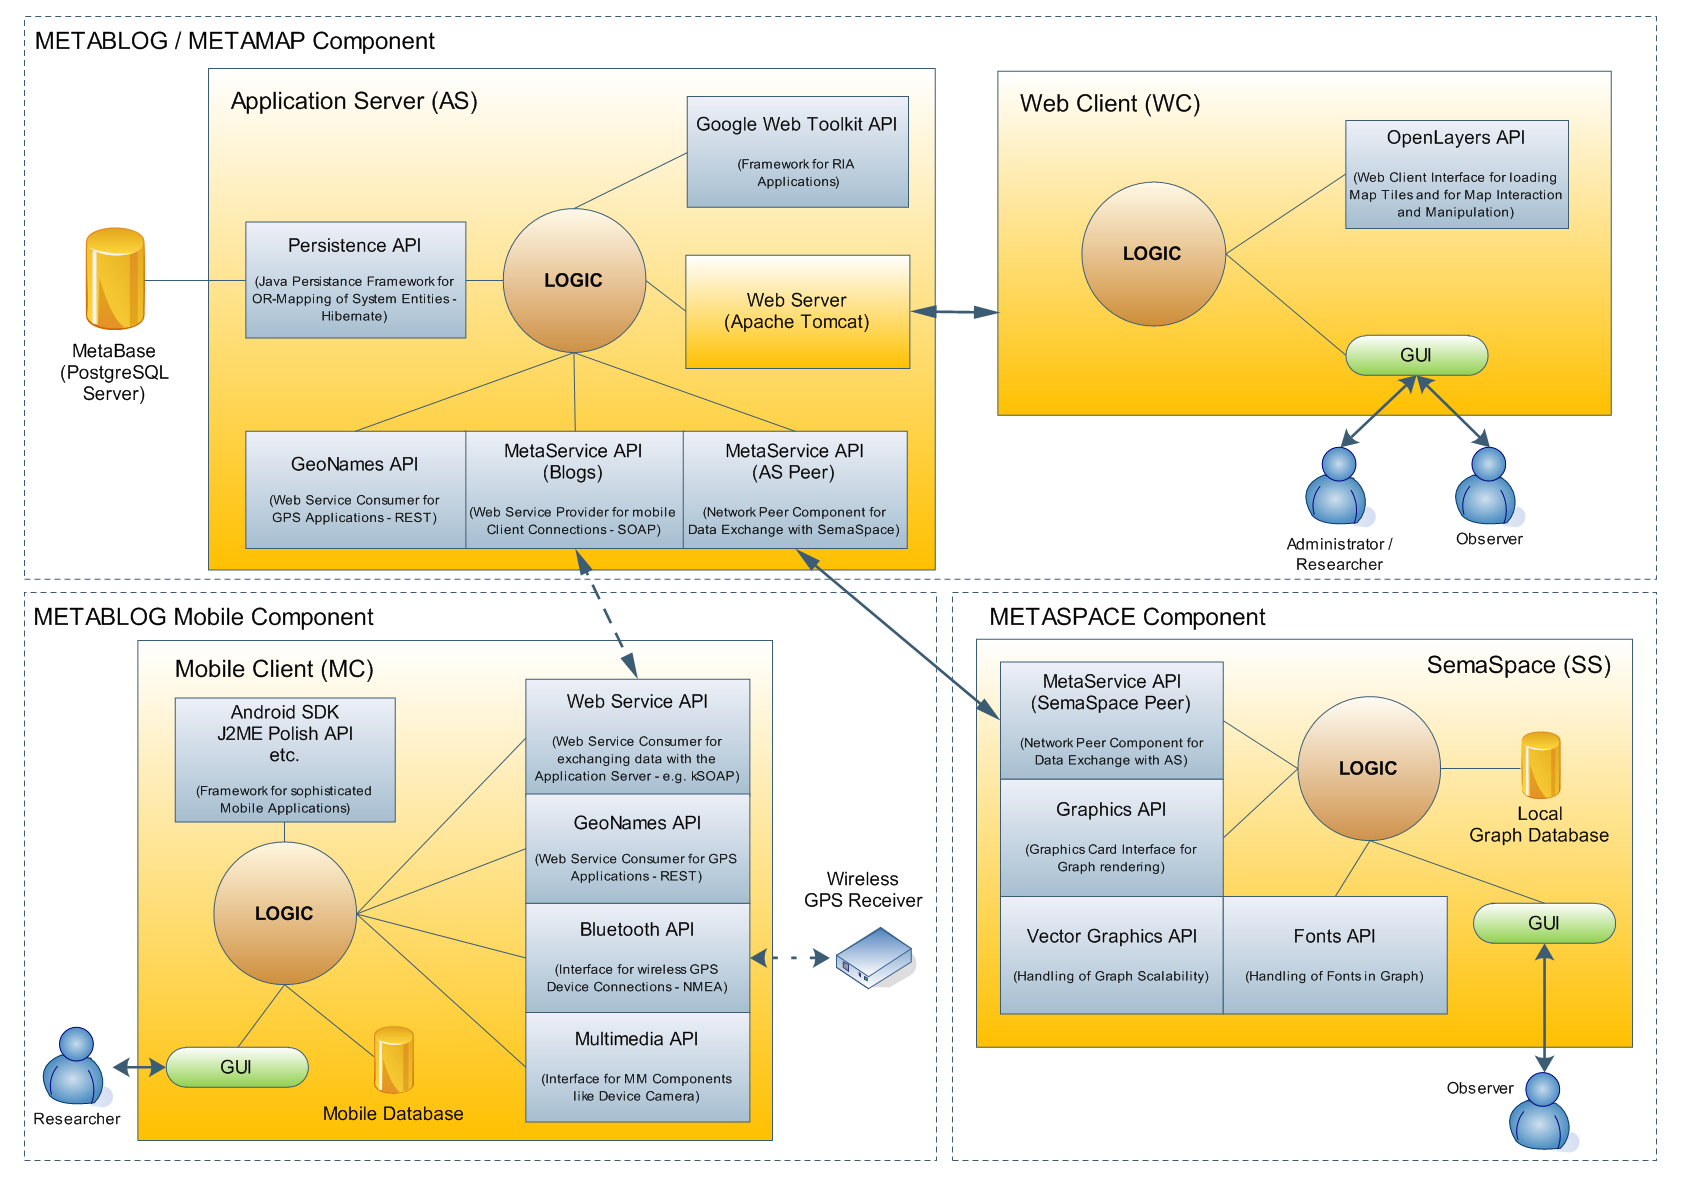
\includegraphics[width=0.85\textwidth]{bin/architecture/component-diagram_update.png}
}

\subsection{interface}
\frame
{
\frametitle{\textbf{realization interface}}
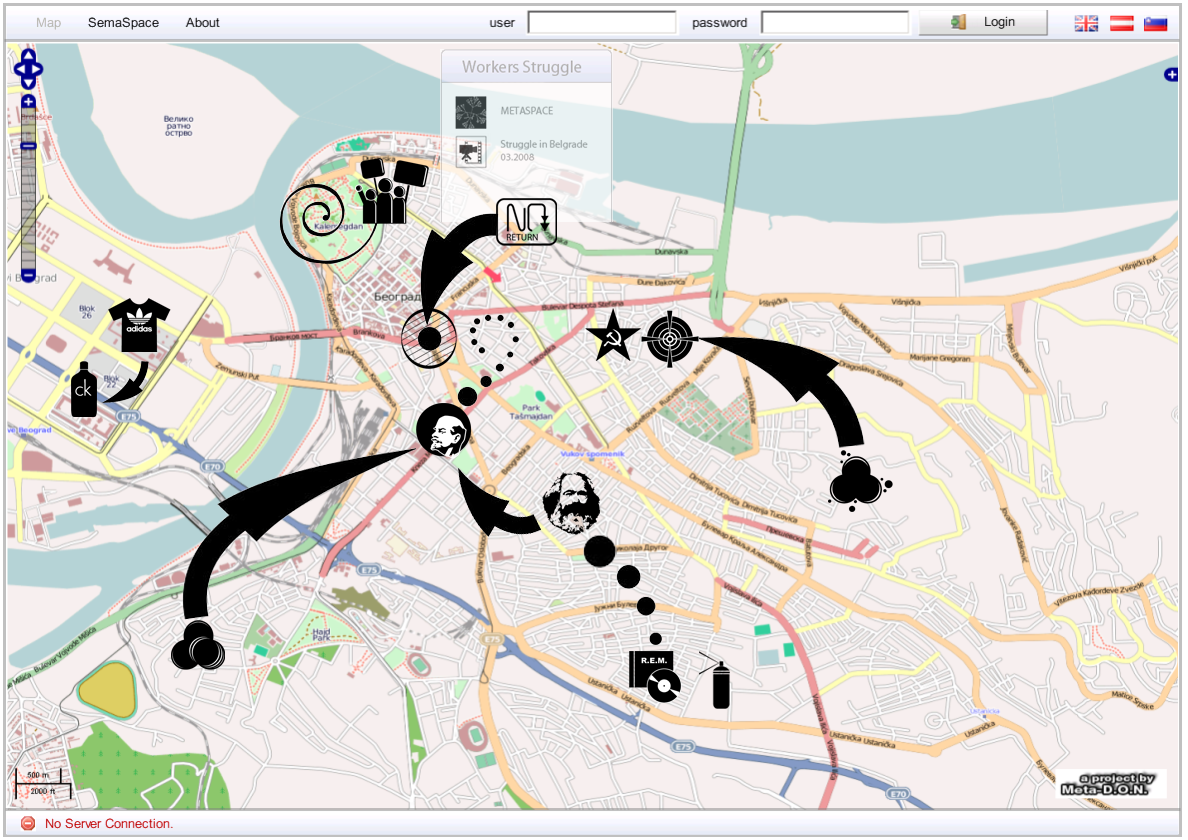
\includegraphics[width=0.85\textwidth]{bin/features/metamap/01_gui_metamap_start_update.png}
}

\frame
{
\frametitle{\textbf{realization interface}}
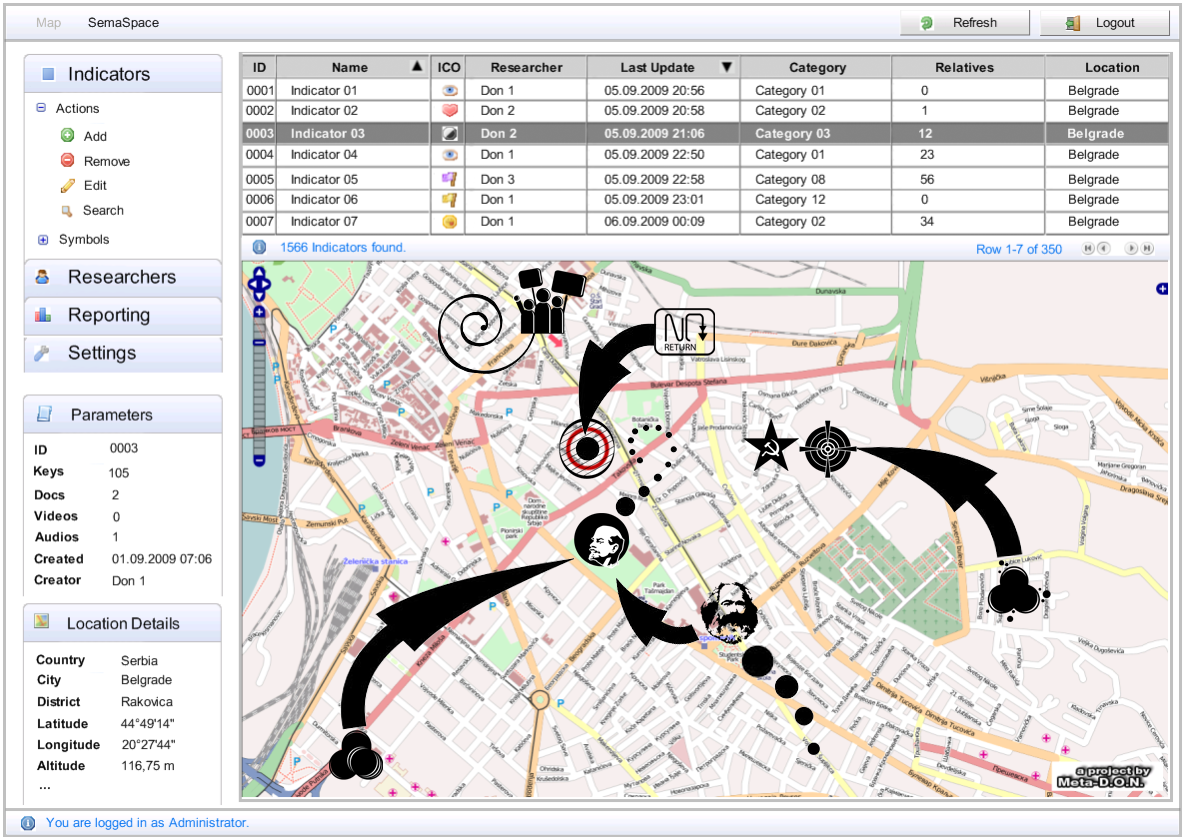
\includegraphics[width=0.85\textwidth]{bin/features/metamap/02_gui_metamap_admin_start_update.png}
}

%%%%%%%%%%%%%%%%%%%%%%%%%%%%%%%%%%%%%%%%%%%%%%%%%%%%%%%%%%%%%%%%%%%%%%%%%%%%%%%%%%%%
%%%%%%%%%%%%%%%%%%%%%%%%%%%%%%%%%%%%%%%%%%%%%%%%%%%%%%%%%%%%%%%%%%%%%%%%%%%%%%%%%%%%

%\section*{Summary}
\frame
{
\frametitle{\textbf{Summary}}
\begin{itemize}
\item \textbf{METANET - Interactive Knowledge Network}
\end{itemize}
}

%%%%%%%%%%%%%%%%%%%%%%%%%%%%%%%%%%%%%%%%%%%%%%%%%%%%%%%%%%%%%%%%%%%%%%%%%%%%%%%%%%%%

\frame[plain]
{
\begin{center}
{\Large\textbf{Thank You.}}
\end{center}
}

\end{document}

%%%%%%%%%%%%%%%%%%%%%%%%%%%%%%%%%%%%%%%%%%%%%%%%%%%%%%%%%%%%%%%%%%%%%%%%%%%%%%%%%%%%


%\begin{beamerboxesrounded}[scheme=alert,shadow=true]{simple.xul}
%\end{beamerboxesrounded}
%\hyperlink{packages<2>}{\beamergotobutton{packages item 2}}


%\frame
%{
%\frametitle{\textbf{title}}
%\begin{itemize}
%\item<1-|alert@1>\textbf{item}
%	\begin{itemize}
%		\item<3-|alert@3> item
%	\end{itemize}
%\item<2-|alert@2>\textbf{item}
%	\begin{itemize}
%		\item<4-|alert@4> item
%	\end{itemize}
%\end{itemize}
%}




